

% Define tab size for indentation
\algrenewcommand\algorithmicindent{2em}%

%%%%%%%%%%%%%%%%%%%%%%%%%%%%%%%%%%%%%%%%%%%%%%%%%%%%%%%%%%%%%%%%
% BLOCKS - \block[]
%%%%%%%%%%%%%%%%%%%%%%%%%%%%%%%%%%%%%%%%%%%%%%%%%%%%%%%%%%%%%%%%

% State, like all blocks ends with \asdend
\algblockdefx[asdstate]{asdstate}{asdend}
{\textbf{State}}{}


% Init
\algblockdefx[asdinit]{asdinit}{asdend}
{\textbf{Init}}{}

\algblockdefx[asdtypes]{asdtypes}{asdend}
{\textbf{Types}}{}

\algdef{SE}[SUBALG]{Indent}{EndIndent}{}{\algorithmicend\ }%
\algtext*{Indent}
\algtext*{EndIndent}

% Upon
\algblockdefx[asdupon]{asdupon}{asdend}
[1][Unknown]{\textbf{Upon} #1 \textbf{Do}}{}
\algblockdefx[asdupontimer]{asdupontimer}{asdend}
[1][Unknown]{\textbf{Upon Timer} #1 \textbf{Do}}{}

% For
\algblockdefx[asdfor]{asdfor}{asdend}
[1][Unknown]{\textbf{Forall} #1 \textbf{Do}}{}

\algblockdefx[asdrepeateveryx]{asdrepeateveryx}{asdend}
[1]{\textbf{Every} #1 \textbf{Do}}{}

% If
\algblockdefx[asdif]{asdif}{asdend}
[1][Unknown]{\textbf{If} (#1) \textbf{Then}}{}

% Else for If
\algcblockdefx[asdelsea]{asdif}{asdelsea}{asdend}
{\textbf{Else}}{}

% Else for Else If
\algcblockdefx[asdelseb]{asdelseif}{asdelseb}{asdend}
{\textbf{Else}}{}

% Else If
\algcblockdefx[asdelseif]{asdif}{asdelseif}{asdend}
[1][Unknown]{\textbf{Else If} (#1) \textbf{Then}}{}

% Interface
\algblockdefx[asdinterface]{asdinterface}{asdend}
{\textbf{Interface}}{}

% Requests
\algblockdefx[asdrequests]{asdrequests}{asdend}
{\textbf{Requests}}{}

% Indications
\algblockdefx[asdindications]{asdindications}{asdend}
{\textbf{Indications}}{}

% Procedure
\algblockdefx[asdprocedure]{asdprocedure}{asdend}
[1][Unknown]{\textbf{Procedure} #1}{}

% Forever
\algblockdefx[asdforever]{asdforever}{asdend}
{\textbf{Forever Do}}{}

%%%%%%%%%%%%%%%%%%%%%%%%%%%%%%%%%%%%%%%%%%%%%%%%%%%%%%%%%%%%%%%%
% STATEMENTS - \statement{} or \statement{}{}
%%%%%%%%%%%%%%%%%%%%%%%%%%%%%%%%%%%%%%%%%%%%%%%%%%%%%%%%%%%%%%%%

% Simple Statements
\newcommand{\asdstatement}[1]{\statenew{#1}}
\newcommand{\asdstatementbold}[1]{\statenew{\textbf{#1}}}

% Trigger
\newcommand{\asdtrigger}[1]{\statenew{\textbf{Trigger} #1}}

% Timer
\newcommand{\asdsetuptimer}[1]{\statenew{\textbf{Setup Timer} #1}}
\newcommand{\asdsetupptimer}[1]{\statenew{\textbf{Setup Periodic Timer} #1}}
\newcommand{\asdcanceltimer}[1]{\statenew{\textbf{Cancel Timer} #1}}

% Call
\newcommand{\asdcall}[1]{\statenew{\textbf{Call} #1}}

% Return - use [] due to xparse
\NewDocumentCommand{\asdreturn}{o}{
	\statenew{\textbf{Return}\IfValueT{#1}{ #1}}
}

% Comment (inline)
\makeatletter
\newcommand{\asdcomment}[1]{
	\parbox[t]{\dimexpr\linewidth-\ALG@thistlm-8em}{
		\strut
		//\space #1
		\strut
	}
}
\makeatother


% Comment (entire line)
\makeatletter
\newcommand{\asdlinecomment}[1]{
		\State \parbox[]{\dimexpr\textwidth-\leftmargin-\labelsep-\labelwidth}{
			//\space #1
		\strut}
}
\makeatother


%%%%%%%%%%%%%%%%%%%%%%%%%%%%%%%%%%%%%%%%%%%%%%%%%%%%%%%%%%%%%%%%
% VALUES
%%%%%%%%%%%%%%%%%%%%%%%%%%%%%%%%%%%%%%%%%%%%%%%%%%%%%%%%%%%%%%%%

% Booleans
\newcommand{\asdfalse}[0]{$false$}
\newcommand{\asdtrue}[0]{$true$}

% Map
\newcommand{\asdmap}[2]{#1{[}#2{]}}

% Set 
\newcommand{\asdset}[1]{$\{$#1$\}$}

%%%%%%%%%%%%%%%%%%%%%%%%%%%%%%%%%%%%%%%%%%%%%%%%%%%%%%%%%%%%%%%%
% Algebraic
%%%%%%%%%%%%%%%%%%%%%%%%%%%%%%%%%%%%%%%%%%%%%%%%%%%%%%%%%%%%%%%%

% Equals (assignment)
\newcommand{\asdassign}[0]{ $\longleftarrow$ }

\algblockdefx[Foreach]{Foreach}{EndForeach}[1]{\For{\textbf{each} #1}}{}

% Equals (comparison)
\newcommand{\asdeq}[2]{#1 $=$ #2}

% Not equals
\newcommand{\asdneq}[2]{#1 $\neq$ #2}

% Exists
\newcommand{\asdexists}[1]{$\exists$ #1}

% Not Exists
\newcommand{\asdnexists}[1]{$\nexists$ #1}

% And
\newcommand{\asdand}[2]{#1 $\wedge$ #2}

% Or
\newcommand{\asdor}[2]{#1 $\vee$ #2}

% Except
\newcommand{\asdexcept}[2]{#1 $\setminus$ #2}

% Union
\newcommand{\asdunion}[2]{#1 $\bigcup$ #2}

% Belongs to
\newcommand{\asdin}[2]{#1 $\in$ #2}

% Not belongs to
\newcommand{\asdnotin}[2]{#1 $\notin$ #2}

% Bottom
\newcommand{\asdbottom}{$ \perp $}

\algnewcommand{\IfThenElse}[3]{% \IfThenElse{<if>}{<then>}{<else>}
  \State \algorithmicif\ #1\ \algorithmicthen\ #2\ \State \algorithmicelse\ #3}


%%%%%%%%%%%%%%%%%%%%%%%%%%%%%%%%%%%%%%%%%%%%%%%%%%%%%%%%%%%%%%%%
% Other
%%%%%%%%%%%%%%%%%%%%%%%%%%%%%%%%%%%%%%%%%%%%%%%%%%%%%%%%%%%%%%%%

\newcommand{\asdnewline}{\hfill\State}

In this section, we discuss the design of the devised overlay network protocol, which aims to build and maintain a latency and capacity-aware tree-shaped network, where capacity represents one, or a combination of, values that denote the node's networking or computing capacity (in our case, we used only bandwidth as each nodes' capacity). We begin by providing the considered system model, then follow with an overview of the mechanisms responsible for building and maintaining the tree, and lastly, we conclude the chapter with a summary and discussion of the protocol.

\subsection{System Model}

The considered system model for this protocol is a distributed scenario composed of nodes connected to the Internet and set up to enable the reception or emission of messages via the Internet (either with an external IP or port-forwarding). We also assume that nodes are spread throughout a large geographical area, have varied capacity values, and are distributed among both Cloud and Edge settings.

Regarding the fault model, we assume that all but a small portion of nodes (also known as the landmarks, which in our model represent data centres) can fail, and when other nodes fail, they do so in a crash-fault manner, stopping the execution of the process along with all emissions and receptions of messages at the time of failure. We assume landmarks have additional fault tolerance provided their privileged infrastructure, or alternatively, we assume that other mechanisms such as replication could be employed to ensure that faulty landmarks are swiftly replaced in case of failure. 
  
Finally, all nodes must run the same software stack with similar configuration settings, installed a priori.

\subsection{Overview}

As previously mentioned, the main objective of the devised protocol is to establish a latency and capacity-aware multi-tree-shaped overlay network, rooted in the previously mentioned landmarks. The motivations for the choice of a tree structure for our network are the following: (1) to map the cloud-edge environment, by rooting the trees on nodes running DCs in the cloud, and setting up the remaining nodes with less capacity in positions where they can be coordinated from the roots (2) to be able to map the heterogeneity of each device in the environment: by biasing the placement of nodes in the tree such that nodes with higher capacity are placed higher in the tree, and nodes with lower capacity are biased towards lower levels of the tree, nodes are used more or less according to their capacity values; (3) the tree structure can be easily employed to perform efficient aggregations, by propagating and merging values (recursively) from the lower to the higher levels of the tree, which is the basis for the aggregation protocol presented in Section~\ref{sec:mon_protocol:tree_agg}; and finally, (4) by leveraging on the tree structure, nodes can propagate information efficiently, given that, in a network composed of N nodes, broadcasts require only N-1 message transmissions to reach all nodes in the network. 

\begin{figure}[htbp]
    \centering
    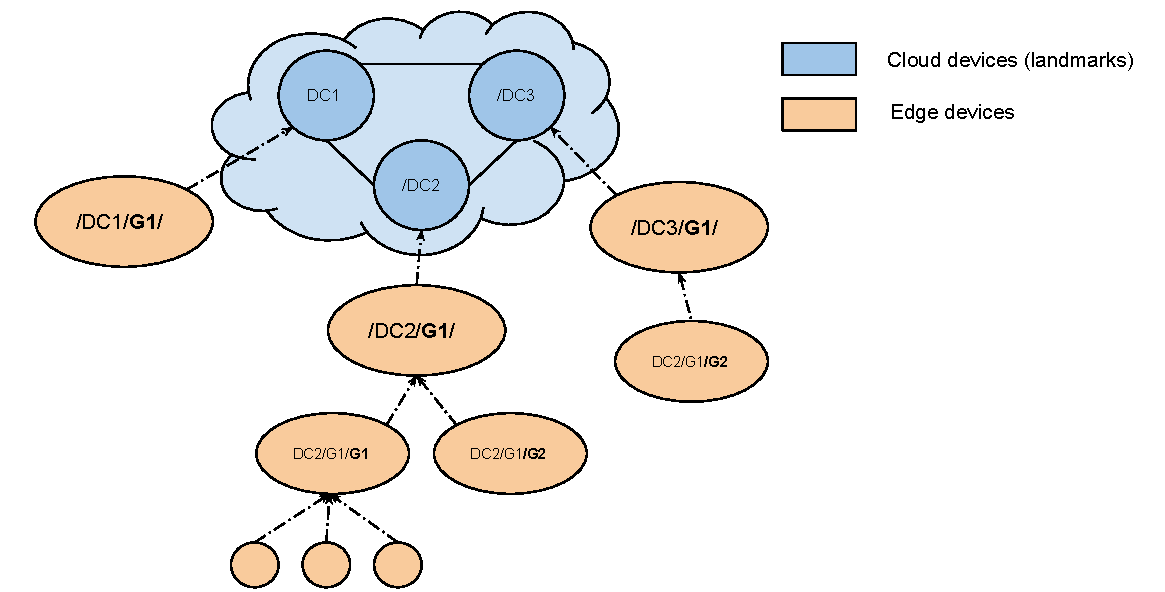
\includegraphics[width=\textwidth]{Chapters/membership/images/DeMMon-overlay-structure.pdf}
    \caption{An example of a network established by the devised protocol (with 3 landmarks)}
    \label{fig:demmon-membership-structure}
\end{figure}

The type of tree structure our protocol aims to establish and maintain is represented in Figure~\ref{fig:demmon-membership-structure}, which, as previously referenced, is composed of multiple interconnected trees. As the reader can note, every node has attributed an identifier, which is the concatenation of the parents' ID with an assigned ID (this mechanism is explained in further detail in Section~\ref{sec:overlay_network:oportunistic_improvement}). The nodes connected to the landmarks (which we refer to as their \textbf{children}) may themselves be the \textbf{parent} of their own children, which would have the landmark as their \textbf{grandparent} (which is the case of ``/DC2/G1/G2'' and ``/DC2/G1/G1''). Intuitively, the \textbf{descendants} of a node are all of its children and children's children, recursively, until the leave nodes. All nodes which share the same parent (\textbf{siblings}) are connected among themselves, forming a \textbf{group}, whose size is biased (but not guaranteed) to be within two configurable upper and lower bounds. Therefore, all nodes have active connections to their parent, children and siblings. The combination of a node's active connections may be called its \textbf{active view} (following the nomenclature introduced in~\cite{Hyparview}). 

The devised algorithm is composed of three main mechanisms: (1) the \textbf{join} mechanism, which aims to establish the initial tree structures, (2) the \textbf{active view maintenance}, responsible for biasing the number of connections for each node and optimizing the connections of each node, (3)  and finally \textbf{passive view maintenance}, responsible for collecting information about peers which are not in the active view, which are used for both fault tolerance and connection optimizations.

\subsubsection{Join mechanism} \label{sec:overlay_network:join}

The Join mechanism is the mechanism responsible for establishing an initial parent connection. It is the aim of this mechanism (from the joining node standpoint), to establish a connection with the node with the least cost possible. This mechanism is the first to be executed by all nodes in the system, and it essentially consists of a depth-first search in the established DeMMon trees. The pseudocode for this algorithm can be observed in Algorithm~\ref{alg:memb:join}. 

% JOIN -----

\begin{algorithm}{}
\caption{Join Protocol} \label{alg:memb:join}
% \setstretch{0.85}
\begin{algorithmic}[1]
    \asdtypes
        \State Node : <lat, parentIP, nrChildren, replied, IP, ID, coords, version, children<IP,  nrChildren\>\>
    \asdend
    \asdstate \label{alg:memb:join:state}
        \State contactedNodes \Comment{collection of all successfully contacted nodes}
        \State nodesToContact set<Node> \Comment{nodes being contacted}
        \State joinTimeouts : dict<Node, time> \Comment{collection of contacted nodes -> timerIDs}
        \State bestPeerLastLevel : Node \Comment{the best peer contacted so far in the join process}
        \State joinReqTimeoutTid : string \Comment{ timerID for join messages}
        \State prevBestP : Node \Comment{ myself}
        \State landmarks : set<IP> \Comment{landmark nodes}
    \asdend

\asdupon[Init(landmarks : set<IP>, selfIP, isLandmark)] \label{alg:memb:join:init}
    \State landmarks \asdassign landmarks 
    \State joinTimeouts, prevBestP \asdassign \{\}, nil
    \IfThenElse{isLandmark}
    {addLandmarkUntilSuccess(landmarks) \label{alg:memb:join:add_land}} 
    {contactNodes(landmarks) \label{alg:memb:join:contact_landm}} 
\asdend


\asdupon[receive(Join<>,sender)] \label{alg:memb:join:recv_join}
    \State sendMessageSideChannel(JoinReply<self.parent, self.node, self.children>, sender) 
\asdend
    
\asdupon[receive JoinReply(<parentIP, node, children>, sender) \&\& measuredLatency(lat)]  \label{alg:memb:join:recv_join_reply}
        \If{\asdin{node.IP}{nodesToContact}} 
            \If{\asdin{parentIP}{Landmarks}}
                \State self.coordinates[getIdx(landmarks, sender)] = lat
            \EndIf
            \State nodesToContact[node.IP].lat \asdassign lat
            \State nodesToContact[node.IP].children \asdassign children
            \State nodesToContact[node.IP].parent \asdassign parentIP
            \State nodesToContact[node.IP].replied \asdassign true
            \State cancelTimer(joinTimeouts[sender])
            \State delete(joinTimeouts, sender)
        \Else
            \State nodesToContact.delete(node)
        \EndIf
\asdend

\asdupon[(forall n $\in$ nodesToContact -> n.replied)] \label{alg:memb:join:cond_go}
    \State contactedNodes.appendAll(nodesToContact)
    \For{node in sortedByLatency(nodesToContact)}
        \If{(\asdnotin{node.IP}{landmarks}) \&\& node.nrChildren == 0} \label{alg:memb:join:verif_children}
            \State continue \Comment{check if node has enough children}
        \EndIf
        \If{prevBestP != nil \&\& (prevBestP.lat $\le$ node.lat || prevBestP.nrChildren < config.minGroupSize)} \label{alg:memb:join:verif_vs_prev}
            \State joinAsChild(prevBestP)
        \Else
            \State prevBestP \asdassign node \label{alg:memb:join:advance}
            \State toContact \asdassign [\asdin{c}{prevBestP.children} -> c.nrChildren > 0]
            \State contactNodes([c.IP for c in toContact])
        \EndIf
        \State return
    \EndFor
    \IfThenElse{prevBestP != nil} 
    {joinAsChild(prevBestP)}  \label{alg:memb:join:join_base_case}
    {abortJoinAndRetryLater()} 
    \State return
\asdend

\asdupon[JoinTimeoutTimer(node) || NodeMeasuringFailed(node)] \label{alg:memb:join:exclusions}
    \IfThenElse{(L in Landmarks)}{abortJoinAndRetryLater()}{delete(nodesToContact[L])} 
\asdend

\asdupon[JoinRequestTimer(p : Node)]
    \If {sender == prevBestP}
        \If{p.parentIP != nil}
            \State prevBestP \asdassign contactedNodes[p.parentIP]
            \State joinAsChild(prevBestP)
        \Else
            \State abortJoinAndRetryLater()
        \EndIf
    \EndIf
\asdend

\asdupon[receive(JoinRequest<>, sender)]
    \State childID \asdassign addChildren(sender) \Comment{new chilren is established, and an ID is generated for it}
    \State sendMessageSideChannel(JoinRequestReply<childID, self>, sender)
\asdend
    
\asdupon[receive(JoinRequestReply<myID, parent>, sender)]
    \If {sender == prevBestP} 
        \State parent \asdassign sender \Comment{Adds Parent is established, join complete}
        \State cancelTimer(joinReqTimeoutTid)
        \State self.ID \asdassign parent.ID + "/" + myID \Comment{Later used in shuffle mechanism}
    \EndIf
\asdend

\asdprocedure[joinAsChild(p : Node)]
    \State joinReqTimeoutTid \asdassign setupTimer(JoinRequestTimer<p>, config.JoinTimeout)
    \State sendMessageSideChannel(JoinRequest<>, p.IP)
\asdend

\asdprocedure[contactNodes(ips : IP{[]})]
    \State nodesToContact \asdassign \{\}
    \State toContact \asdassign [Node<0,nil,0,false,ip,false,[]> for ip in ips]
    \For{n in toContact}
        \State nodesToContact[n] \asdassign n
        \State MeasureNode(n) 
        \State sendMessageSideChannel(JoinMessage<>, n)
        \State joinTimeouts[n] \asdassign \asdassign setupTimer(JoinTimeoutTimer(n), config.JoinTimeout)
    \EndFor
\asdend

\end{algorithmic}
\end{algorithm}


The first step of the algorithm (line~\ref{alg:memb:join:state}) is to initialize the state of the joining node, that is materialized by: (1) a map called \textit{contactedNodes} of type ``Node'', containing all nodes contacted successfully in the join process (indexed by a string representation of their IP), (2) a collection named \textit{nodesToContact} of type ``Node'' containing the nodes to yet to contact in the join process, (3) a map of timer IDS indexed by strings, containing the timer IDS for each contacted node, named \textit{joinTimeouts}, (4) a variable called \textit{prevBestP} containing the best (lowest latency) node contacted so far in the join process, (5) a variable named \textit{joinReTimeoutId}, containing a timer id for a timer used as a timeout for the chosen node in the join process, (6) a variable of type ``Node'' denoting the peer executing the protocol, and finally (7), a set containing the landmarks of the network, named \textit{landmarks}. The type ``Node'' is a collection of attributes regarding a certain physical node, composed of: (i) latency measured, (ii) its current parent, (iii) number of children, (iv) whether the node replied to the message, (v) its IP, (vi) an array of coordinates (denoting its measured latency to each landmark, used in passive view maintenance mechanism), and finally, (vii) an array of its childrens' IP and their respective number of children.
 
The procedures that are used to join the tree differ regarding if the node is a landmark or not (which is a configuration parameters provided at the setup of a node): in the case of landmarks, these attempt to repeatedly establish a connection with other landmarks through the emission of a special message. Landmarks that receive this message always send a reply and establish a connection to the sender of the message (line~\ref{alg:memb:join:add_land}). Any joining landmark only stops sending messages to other landmarks when the respective reply is received and an outgoing connection is established.

Nodes that are not landmarks begin the process of finding their initial parent in the DeMMon tree. This process is initiated by measuring the current latency and sending a JOIN message (via a temporary TCP channel) to the landmarks. For each message sent, a timer is created, and its ID is stored in the \textit{joinTimeouts} map (line~\ref{alg:memb:join:contact_landm}). Whenever a node receives this JOIN message, it sends a JOINREPLY message back to the original sender containing: its parent, itself, and its children (line~\ref{alg:memb:join:recv_join}).

During the wait process, the joining node waits for either the responses from the contacted nodes, for any timer in the \textit{joinTimeouts} map to trigger, or for any failed latency measurements. In the second and third cases, the contacted node is excluded from the join process, and it is resumed as normal (line~\ref{alg:memb:join:exclusions}). In case there are no nodes left to resume the join process, or if the excluded node is a landmark, then the node waits a configurable amount of time until attempting to re-join the overlay again. 

If the contacted node has not failed, and the joining node receives the JOINREPLY (line~\ref{alg:memb:join:recv_join_reply}), it checks if it came from a timed-out node or from any node whose parent was not contacted in the join process (e.g. if the contacted node changed parent during the join process), if any of these situations occurs, then the message is discarded. If none of these situations occurs, the message is not discarded, and the information contained in the JOINREPLY message is stored in the \textit{contactedNodes} map.

Whenever the joining node has either received the JOINREPLY messages from all contacted nodes or they have been excluded from the join process, it evaluates all the successfully contacted nodes attempting to find the contacted node with the lowest latency that is a suitable parent (by suitable, we mean a node that already has children or is a landmark). This procedure is performed by sorting the nodes in ascending order of measured latency and performing the following verifications:

\begin{enumerate}
    \item Verify if the node already has any children or if the node is a landmark (landmarks can become parents of any node, except other landmarks) (line~\ref{alg:memb:join:verif_children}). If it is neither of these situations, then the node is excluded from the join process. 
    
    \item Verify if there was a node already contacted previously which was a suitable parent and had lower measured latency. In case there was, the joining node sends a \textsc{JoinRequest} message (requesting to be its child), sets up a \textit{JoinRequestTimer} for the lower latency node, and stops the join process. (line~\ref{alg:memb:join:verif_vs_prev})

    \item Verify if the current node has both enough children and has the lower latency when compared to the best previous last node. If so, then the joining node assigns it as its best node so far and starts a new recursive step by sending JOIN messages and measuring the latency to the children of that node which themselves have more than one children (line~\ref{alg:memb:join:advance}). Note that if none of the current nodes' children is a suitable parent (i.e. have no children themselves), then the condition in line~\ref{alg:memb:join:cond_go} is triggered, and the joining node requests the current best node to be its parent.
    
    \item If none of the verified peers was suitable to start a new recursive step (either because it had no children or had higher latency when compared to a previously contacted node), then the node joining node sends a \textsc{JoinRequest} to the best previously contacted node (in terms of latency), and sets up a \textit{JoinRequestTimer} for it  (line~\ref{alg:memb:join:join_base_case}). 
\end{enumerate}



The node that receives this \textsc{JoinRequest} message replies with a \textit{JoinRequestReply} and adds the node to its children by attempting to establish an outbound connection to it. Then, the join process is concluded with the reception of the \textit{JoinRequestReply} and the establishment of the connections between the two nodes. If, however, the \textit{JoinRequestTimer} timer triggers while waiting for the response, the node will fall back to the parent of the selected node, (and do so recursively, in case the parent of the current node failed as well, until reaching the landmark of that branch).

\subsubsection{Active view maintenance} \label{sec:overlay_network:active_view_maint}

The second mechanism of the devised membership algorithm, called active view maintenance, is the mechanism responsible for maintaining the size of the groups and optimizing the nodes' active connections (when possible). This mechanism is performed by each parent periodically when their group size is above a certain threshold size, through the emission of messages to one (or more) of its children, proposing they should connect to another provided parent. The nodes chosen to be the new parents are chosen using latency measurements and node capacity as heuristics, obtained via periodic transmission from every child to their parent. 

The pseudocode for this mechanism is presentend in Algorithm~\ref{alg:memb:active_view_maint}, and it starts by defining the necessary state to execute it, starting by the nodes' active view (parent, children, and siblings), and an auxiliary map of sets, named \textit{childrenLatencies}, which holds the latencies of each children to every other children. (lines~\ref{alg:memb:active_view_maint:state_start}-\ref{alg:memb:active_view_maint:state_end}). 

\begin{algorithm}
    \caption{Membership protocol (Active view Optimization)} \label{alg:memb:active_view_maint}
    % \begin{multicols}{2}
    % \setstretch{0.85}
    \begin{algorithmic}[1]
        \asdstate
            \State parent \Comment{defined in join} \label{alg:memb:active_view_maint:state_start}
            \State children \Comment{defined in join} 
            \State siblings  
            \State childrenLatencies : dict<string:dict<string:number>> \label{alg:memb:active_view_maint:state_end} \Comment{Holds the latencies of each children to every other children}
        \asdend

        \asdrepeateveryx{config.updatePeriodicity} \label{alg:memb:active_view_maint:update}
            \If{parent != nil}
                \State sLatencies \asdassign set()
                \For{sibling in siblings}
                    \State sLatencies.append(<sibling.IP,sibling.measuredLatency)
                \EndFor
                \State sendMessage(UpdateChildStatus<children, siblingLatencies>, parent)
            \EndIf
            \For{child in chidren}
                \State sendMessage(UpdateParentStatus<self, chidren \\ child>)
            \EndFor
        \asdend \label{alg:memb:active_view_maint:update_end}

        \asdupon[receive(UpdateParentStatus<parent, children>, sender)] 
        \label{alg:memb:active_view_maint:update_recv_par}
            \If{sender == parent.IP}
                \State parent \asdassign parent
                \State self.ID \asdassign parent.ID + "/" + myID
                \State grandParent \asdassign grandParent
                \State siblings \asdassign siblings
                \State measureSiblingLatency(siblings)
            \EndIf
        \asdend

        \asdupon[receive(UpdateChildStatus<child, childSiblingLatencies>, sender)]\label{alg:memb:active_view_maint:update_recv_chi}
            \If{children[sender] != nil}
                \State children[sender]\asdassign child
                \State childrenLatencies[sender] \asdassign childSiblingLatencies
            \EndIf
        \asdend
    
    % \end{algorithmic}
    % \columnbreak
    % \begin{algorithmic}
    
        \asdrepeateveryx{config.evalGroupSize} \label{alg:memb:active_view_maint:update_eval}
            \If{len(children) <= config.maxGroupSize}
                \State return
            \EndIf
            \State childrenLatValues \asdassign set()
            \For{c1 in children} \label{alg:memb:active_view_maint:update_eval_merge_start}
                \For{<c2, lat> in childrenLatencies[c]}
                    \If{lat - c1.measuredLatency > d.config.maxLatDowngrade}
                        \State continue
                    \EndIf
                    \IfThenElse{c1.cap > c2.cap}
                    {childrenLatValues.add(<c1,c2,lat>)}
                    {childrenLatValues.add(<c2,c1,lat>)}
                \EndFor
            \EndFor \label{alg:memb:active_view_maint:update_eval_merge_finish}
            \State kickedNodes, newParents \asdassign set(),set()
            \State pChildren \asdassign dict<string,set<Node{>}{>} \Comment{set of potential children for each children}
            \State sortByLatency(childrenLatValues)
            \State idealGroupSize \asdassign config.maxSize - config.MinGroupSize
            \For{<c1,c2,lat> in childrenLatValues}
                \If{len(children) - len(kickedNodes) <= config.maxSize} \label{alg:memb:active_view_maint:check_done_1}
                    \State break
                \EndIf
                \If{\asdin{c1}{kickedNodes} || \asdin{c2}{kickedNodes} ||  \asdin{c1}{newParents}} \label{alg:memb:active_view_maint:check_done_2}
                    \State continue
                \EndIf
                \If{c1.nrChildren == 0 \&\& newParents[c1] == nil} \Comment{Node is not yet a parent}
                    \State pChildren[c1] \asdassign pChildren[c1] + c2 \label{alg:memb:active_view_maint:add_set}
                    \If{len(pChildren) == config.MinGroupSize}
                        \For{potentialChild in pChildren[c1]} \label{alg:memb:active_view_maint:kick_set_start}
                            \State newParents \asdassign newParents + c1
                            \State kickedNodes \asdassign kickedNodes + potentialChild
                            \State send(OptimizationPropose<c1>, potentialChild)
                        \EndFor
                        \For{<nIP,pontentialChildrenTmp> in pChildren}
                            \State pontentialChildrenTmp.deleteAll(pChildren[c1])
                        \EndFor
                        \State pChildren[c1] \asdassign set<Node> \label{alg:memb:active_view_maint:kick_set_end}
                    \EndIf
                \Else \label{alg:memb:active_view_maint:kick_already_parent}
                    \State kickedNodes \asdassign kickedNodes + c2
                    \State send(OptimizationPropose<higherCapNode>, lowerCapNode)
                \EndIf    
            \EndFor
        \asdend

        \asdupon[receive(OptimizationPropose<newParent>, sender)] \label{alg:memb:active_view_maint:opt_propose_recv}
            \If{sender == parent}
                \State send(OptimizationProposeRequest<sender>, newParent)
            \EndIf
        \asdend

        \asdupon[receive(OptimizationProposeRequest<p>, sender)] \label{alg:memb:active_view_maint:opt_propose_req_recv}
            \If{ p == parent \&\& sender in siblings} \Comment{ parent issuing the message is my parent}
                \State addChild(sender)
                \State send(OptimizationProposeRequestReply<true,p>, sender)
            \Else
                \State sendSideChannel(OptimizationProposeRequestReply<false,p>, sender)
            \EndIf
        \asdend

        \asdupon[receive(OptimizationProposeRequestReply<reply,p>, sender)] \label{alg:memb:active_view_maint:opt_propose_req_reply_recv}
            \If{parent == p}
                \If{reply}
                    \State sendMessageAndDisconnectFrom(DisconnectMessage<>, parent)
                    \State addParent(sender)
                \EndIf
            \Else
                \State sendMessageTemporaryConn(DisconnectMessage<>, p)
            \EndIf
        \asdend

    \end{algorithmic}
% \end{multicols}
\end{algorithm}

This mechanism starts with the periodic propagation of information from the parent to its children and vice versa. As denoted in lines~\ref{alg:memb:active_view_maint:update}-\ref{alg:memb:active_view_maint:update_end}, each parent transmits to its children a list of its current children (the siblings, from the children's point of view). Then, the children nodes measure their latencies to each of their siblings, and propagate the obtained latency values back to the parent. When this information is received (lines~\ref{alg:memb:active_view_maint:update_recv_par} and~\ref{alg:memb:active_view_maint:update_recv_chi}), it is merged into their respective local view for later use.

The second part of this mechanism is responsible for maintaining the group sizes by creating new parents or by sending children to already created groups (line~\ref{alg:memb:active_view_maint:update_eval}). This mechanism is triggered periodically but only executes if the number of children of a  node (denoted the \textit{proposer} node) exceeds the configured maximum number of children per parent. In this mechanism, a \textit{proposer} node proposes to one of its children (denoted node \textit{C1}) a change of parent to one of the \textit{proposers'} children (denoted the \textit{C2} node).


When triggered, the proposer node begins by merging all of its received latency pairs into a single set, where the node with the highest capacity is the first node of each pair. While doing so, it discards any new edges which would otherwise lower the overall latency of the system by a larger than configured amount (lines~\ref{alg:memb:active_view_maint:update_eval_merge_start}-\ref{alg:memb:active_view_maint:update_eval_merge_finish}). Then, the \textit{proposer} node iterates over the merged edge pairs set by ascending order of latency cost, performing the following steps:

\begin{enumerate}
    \item If the number of current children minus the number of nodes already sent to lower levels is lower than the configured maximum group size, then the mechanism has achieved its purpose, and the \textit{proposer} node concludes the mechanism (line~\ref{alg:memb:active_view_maint:check_done_1})
    
    \item If any of the two nodes were already sent to lower levels of the tree in previous steps, then the current edge is skipped (line~\ref{alg:memb:active_view_maint:check_done_2}).
    
    \item Then, if the node with higher capacity of the edge pair has no children yet, the lower capacity node is added to its \textit{possibleChildren} set (line~\ref{alg:memb:active_view_maint:add_set}). When this set has the same size as the minimum configured group size, then the node issues \textsc{OptimizationPropose} messages for each node of the \textit{possibleChildren} set, and removes each child from every other node's potential children (lines~\ref{alg:memb:active_view_maint:kick_set_start}-\ref{alg:memb:active_view_maint:kick_set_end}). Alternatively, if the higher capacity node already is a parent (either because some nodes were already chosen to form its group, or because it was already a parent previously), then the coordinator node issues an \textsc{OptimizationPropose} message to it (line~\ref{alg:memb:active_view_maint:kick_already_parent}).
\end{enumerate}

When node \textit{C1} receives an \textsc{OptimizationPropose} message, containing a new proposed parent (line~\ref{alg:memb:active_view_maint:opt_propose_recv}), it verifies that the message was sent by its current parent, discarding it if it is not. After this, it sends an \textsc{OptimizationProposeRequest} message containing itself and the \textit{proposer} to the \textit{C2} node, indicating it wishes to become its child. When the proposed parent receives this message (line~\ref{alg:memb:active_view_maint:opt_propose_req_recv}), it verifies that the \textit{proposer} node is still its parent and that node \textit{C1} is also its sibling, if yes, then it adds the node as its new child, and replies with an \textit{OptimizationProposeRequestReply}. This message contains a boolean flag, signalling if the node was added as a child or not. When this message is received (line~\ref{alg:memb:active_view_maint:opt_propose_req_reply_recv}) by node \textit{C1}, it also verifies that the \textit{proposer} node is still its parent, aborting the process if it is not, and adds the proposed node as its parent.

After this process is complete, if not aborted, the \textit{C2} node becomes the parent of node \textit{C1}, and the \textit{proposer} node has fewer children, reducing its group size towards the configured maximum (as the \textit{proposer} node only executes this mechanism if its children number exceeds the configured amount). Furthermore, when possible, node \textit{C1} obtains a new node with lower latency than its current latency to the \textit{proposer} node, effectively improving the overall overlay cost, while maintaining group sizes within bounds.

It is important to note that since the mechanism limits the latency downgrade for each new parent connection, it does not guarantee that group sizes are bounded. Although it would be possible to bound the number of nodes per group if this condition were ignored, then this mechanism would conflict with the third mechanism, described in Section~\ref{sec:overlay_network:oportunistic_improvement}

A final mechanism employed in the management of the active view maintenance that is omitted from the pseudocode is responsible for ensuring that groups sizes do not become too small. In summary, every node periodically verifies the number of peers that are its siblings, if this number is lower than a certain (configurable) bound, the node ``rolls a dice'' (essentially generates a random number and verifies if it is lower/above a certain configurable threshold) to decide if it should abandon the current group in favour of joining its grandparents'. If the dice roll is positive, then the node sends a message to its grandparent asking to become its child. When the grandparent receives this message, it verifies if the exchange causes a loop in the tree and adds the node to its children if it does not. Then, it notifies the sender of the message by sending a message reply containing a boolean value representing if the sender node was accepted as a child or not. 

 It is important to mention that the aforementioned threshold of the ``dice roll'' (and consequently the probability of the node remaining in the current group) changes as a function of the size of the group, decreasing proportionally to the difference between the configured minimum group size and the current nodes' group size.

\subsubsection{Passive view maintenance \& Oportunistic improvement} \label{sec:overlay_network:oportunistic_improvement}

The third mechanism of the devised membership algorithm is called ``Passive view maintenance \& Oportunistic improvement'', and as its name suggests, it is responsible, in each node, for creating and maintaining an auxiliary pool of nodes in the overlay which are not descendants of the local node. This pool serves two purposes: the first is to enable fault tolerance in the overlay without having to rely on the landmarks, the second is to enable the self-improvement of the overlay, through parent exchanges toward ``closer'' parents (according to latency values). 

There are three components of the Node type (the ID, Coordinates and the version of each node) which were present in the pseudocode of the previous mechanisms, but their explanation was omitted given they are only relevant to the behaviour of the this mechanism. We now explain each in detail and how they are obtained:

\begin{enumerate}
    \item The \textbf{ID} of each node is a collection of string segments, where each node's ID is the concatenation of every segment of every ascendant of the node with its own segment. Each node's segment is generated by each parent whenever a new node requests to be its child. An example of the resulting IDS can be observed in Figure~\ref{fig:demmon-membership-structure}, where, for example, all nodes that are descendants of the node with ID ``DC2'', begin their ID with ``DC2'' (e.g. ``DC2/G1''). In this case, the ID is made up of the segments: ``DC2'' and ``G1''. This hierarchical ID structure gives each node enough information to evaluate if any other node in the overlay is its descendant (by verifying if one of ID is contained in the other), therefore allowing nodes to evaluate if a change of parent in the overlay would cause a cycle in the tree. This ID structure also allows nodes to check the level of any node, as the number of segments of an ID is the same as the level of that node in the tree (where landmarks are the root of the tree).
    
    \item The \textbf{coordinates} of each node is an array of integers, where each position contains the obtained latency toward the corresponding landmarks. These coordinates are used as a heuristic for measuring the distance to new nodes in the passive view (to be potential parents).
    
    \item The \textbf{version number} of a node is a monotonic integer that is incremented at every ID change and child addition or removal. The versions number allow nodes to replace outdated entries in their passive views. For example, if a node switches parent, it also changes its ID (and increases its version number). In this situation, other nodes must update their passive views to reflect this change, this is important as it may prevent them from measuring the latency to a node that could potentially be an incompatible parent because it would cause a cycle in the tree previously (i.e., before the change of its ID).
\end{enumerate}

With these concepts explained, we now present the pseudocode for the mechanism (Algorithm~\ref{alg:memb:passive_view_maint}). Similar to previous algorithms, the first lines declare the necessary state maintained by each node to execute the mechanism, which is composed of a set of nodes materializing the passive view of the node (line~\ref{alg:memb:passive_view_maint:state}). In the following lines, we may observe the mechanism for filling this set. This mechanism is a periodic procedure triggered at pre-configured intervals which causes the emission of a new random walk message (line~\ref{alg:memb:passive_view_maint:walk_trig}), the created random walk message contains (1) a random sample of nodes from the emitting node's passive view and active view, (2) the original sender's ID, and (3) an integer representing the messages' time-to-live (TTL). This message is then sent to a node that is not a descendant of the sender.

\begin{algorithm}
\caption{Membership protocol (Oportunistic Optimization)}
\begin{algorithmic}[1]
    

    \asdstate
        \State eView : set<Node>
    \asdend

    \asdrepeateveryx{config.RandWalkPeriodicity}
        \State ascNeighs, allNeighs = set
        \State ascNeighs = ascNeighs + parent + siblings
        \State allNeighs = allNeighs + ascNeighs + children
        \State sample = getRandSample(eView + allNeighs, config.NrPeersToMergeRandWalk)
        \State sendMessage(RandomWalk<sample, config.RandWalkTTL, self.ID, self.IP>, getRand(ascNeighs))
    \asdend

    \asdrepeateveryx{config.OportunisticOptimizationTimeout}
        \State toMeasureRand = getRandSample(eView, config.NrPeersToMeasureRandom)
        \State toMeasureBiasedOpts = sortByEuclideanDist(eView / toMeasureRand)
        \State toMeasureBiased = getRandSample(toMeasureBiasedOpts, config.NrPeersToMeasureRandom)
        \For p in toMeasureRand:
            \State measurePeer(p)
        \EndFor
        \For p in toMeasureBiased:
            \State measurePeer(p)
        \EndFor
    \asdend


    \asdupon[receive( RandomWalk<sample, ttl, nID, orig>, sender)]
        \State stepsTaken = config.RandWalkTTL - ttl
        \State nrToAdd = config.NrPeersToMergeRandWalk
        \State nrToMerge = config.NrPeersToMergeRandWalk
        \State ascNeighs, allNeighs = set(), set()
        \State ascNeighs = ascNeighs + parent + siblings
        \State allNeighs = allNeighs + ascNeighs + children

        \If{stepsTaken < config.NrStepsToIgnore}:
            \State nrToMerge = 0
        \EndIf

        \State toAdd = getRandSample(excludeDescendantsOf([eView + allNeighs] / sample),nID), nrToAdd)
        \State toRemoveFromSample = getRandSample(sample, nrToMerge)
        \State sample = sample / toRemoveFromSample
        \State sample = sample + toAdd
        \State target = getRand(excludeDescendantsOf(allNeighs, nID)
        \If{target == nil || ttl == 0}
            \State sendMessageSideChannel(RandomWalkReply<sample>, orig)
        \Else
            \State sendMessage(RandomWalk<sample, ttl-1, nID, orig>, getRandom(ascNeighs))
        \EndIf
        \State eView = excludeDescendantsOf(toRemoveFromSample, self.ID)  + eView
        \State eView = eView / allNeighs
        \State eView = eView[:config.MaxEViewSize]
    \asdend

    \asdupon[peerMeasured(p, latency)]
        \State latencyImprovement := parent.measuredLatency - Latency
        \If{latencyImprovement >= config.MinLatencyForImprovement}
            \State sendMessageSideChannel(OportunisticImprovementReq<self>,p)
        \EndIf
    \asdend


    \asdupon[receive(OportunisticImprovementReq<p>,sender)]
        \If{isDescendent(p.ID,self) or parent == nil}
            \State sendMessageSideChannel(OportunisticImprovementReqReply<false>,sender)
        \Else
            \State addChildren(sender)
            \State sendMessageSideChannel(OportunisticImprovementReqReply<true>,sender)
        \EndIf
    \asdend

    \asdupon[receive(OportunisticImprovementReqReply<answer>,sender)]
        \If {answer} 
            \State addParent(sender)
        \EndIf
    \asdend

    \asdprocedure[isDescendentOf(nodeID, PotentialDescID)]
        \State return PotentialDescID.Contains(nodeID)
    \asdend

\end{algorithmic}
\end{algorithm}

Whenever this message is received (line~\ref{alg:memb:passive_view_maint:walk_rec}), if it has travelled more than a certain (configurable) number of hops, then the receiving node removes a (also configurable) number of nodes from the sample. Conversely, if the message has not yet travelled the number of hops, the previous step is skipped. After this, the node merges the removed nodes (if there are any) into his passive view and adds a random sample of nodes from his own passive and active view to the sample. If the configured maximum sample size is exceeded, then a number equal to the number of inserted nodes is discarded from the sample at random (lines~\ref{alg:memb:passive_view_maint:walk_rec_merge_start}-\ref{alg:memb:passive_view_maint:walk_rec_merge_end}). The intuition behind skipping a certain number of hops before removing nodes from the sample is to promote nodes collecting information from nodes further away in number of hops from the source of the random walk. After this, the message TTL is decreased by one and its value is evaluated: if the TTL of the message is higher than 0, then the node forwards the message to a random node from its active view that is not a descendant of the original sender (descendants are excluded by verifying if their ID is not contained in the original senders'). If there is no valid target to forward the message to, then the node sends (via a temporary connection) a \textsc{RandomWalkReply} message to the original sender of the random walk with the sample (lines~\ref{alg:memb:passive_view_maint:walk_rec_send}-\ref{alg:memb:passive_view_maint:walk_rec_send_end}). 

Whenever a node receives a \textsc{RandomWalkReply} it merges the received sample with its passive view, excluding all of its descendants and nodes in the active view (lines~\ref{alg:memb:passive_view_maint:walk_reply_recv_start}-\ref{alg:memb:passive_view_maint:walk_reply_recv_end}).

As the overlay evolves with time, the passive views of nodes fill with nodes that are not descendants of the node in question, meaning they are suitable for latency optimizations and fault recovery (in case a parent dies). The (periodic) procedure responsible for evaluating these nodes can be observed in lines~\ref{alg:memb:passive_view_maint:eval_nodes}, where the node selects two (configurable) samples from the passive view to evaluate: a random sample and a sample based on the euclidean distance of the coordinate pair. Each node selected for this sample (candidates) must satisfy the following conditions (lines~\ref{alg:memb:passive_view_maint:opt_verification_1} and~\ref{alg:memb:passive_view_maint:opt_verification_2}): 

\begin{enumerate}
    \item Have more than one direct descendant (i.e. more than one child). 
    
    \item If the candidates' level (obtained from the ID) is lower than the measuring nodes' and the measuring node has more than 0 children, then the candidate is excluded. This prevents nodes with multiple children from going down in levels and instead favours nodes with no children ``climbing'' to higher levels of the tree.
\end{enumerate}

After the measurements are issued, whenever a \textsc{peerMeasured} event is triggered (line~\ref{alg:memb:passive_view_maint:peer_measured}), the node compares the current latency of its parent with the measured nodes' latency: if that latency is lower than the current parents' latency by a configurable threshold, then the measuring node will send an \textsc{OportunisticImprovementReq} message to the measured node. When the measured node receives this message (line~\ref{alg:memb:passive_view_maint:oport_msg_recv}), it checks that the receiving node is not a descendant of the sender (to prevent the creation of loops in the tree) and replies with an \textsc{OportunisticImprovementReqReply} message containing a boolean value representing whether the node was accepted as a child or not.

When this message is received, (line~\ref{alg:memb:passive_view_maint:op_msg_reply_recv}), if the exchange was accepted, the node disconnects from the parent node (via a special message), establishes a connection to the new parent, and updates its own ID and version.

\subsubsection{Fault tolerance}

Fault tolerance in this protocol is triggered whenever a node detects its parent has failed. This can be achieved either by the PHI-accrual failure detector provided by the Node Watcher (Section~\ref{sec:Node-Watcher}) or by the failure of a TCP connection that triggers a notification to the protocol. Whenever this occurs, the node first attempts to fall back to its grandparent (provided via the periodic information in Section~\ref{sec:overlay_network:active_view_maint}), if this fails, it falls back to any node in its passive view that is not a descendant.

When a node falls back to another node, it sends a \textsc{FaultRecovery} message containing its ID and sets up a timeout timer for each fault recovery attempt. Nodes that do not reply to \textsc{FaultRecovery} messages within the specified timeout are considered to be failed and are removed from the passive view. If this view becomes empty, then the node starts the join mechanism again (Section~\ref{sec:overlay_network:join}).

\subsection{Summary}

In this section, we provided a detailed explanation of the behaviour of the membership protocol. We began by explaining how nodes join the network using a greedy depth-first search to find a suitable low-latency node in the network with more than zero children. Then, after this low-latency parent is established, we described how information between nodes and their parents is exchanged over time and how the parent node coordinates with its children in an attempt to maintain the group size within a certain bound and (when possible) reduce the systems' latency.

Lastly, we explained how nodes obtain information about other random nodes in the network and how that information is employed to perform both latency optimizations that reduce the total overlay network latency. Lastly, we covered fault recovery in the protocol, which occurs whenever the parent of a certain node crashes.